\section{Bayesian Analysis}
\label{sec:bayesian}

\subsection{Priors and Posterior}
\label{sec:bayes_prior}
\emph{In short: uniform bounded priors on twelve parameters; with $\sim2\times10^4$ candidates the posterior is dominated by the likelihood.}
Bayes' theorem combines the likelihood of Eq.~\eqref{eq:likelihood} (Sec.~\ref{sec:model}) with a prior $\pi(\theta)$ into the posterior
\begin{equation}
p(\theta\mid D)=\frac{\mathcal{L}(D\mid\theta)\,\pi(\theta)}{p(D)},
\label{eq:bayes}
\end{equation}
The priors are uniform, with independent ranges except for the ordering of the background slopes: $N_s,N_b\in(0,5N)$ with $N=19{,}731$, $A,A_b\in(-1,1)$, $\mu\in(5260,5310)\,\MeV$, $\sigma\in(3,40)\,\MeV$, $\lambda_1^{\pm}\in(10^{-5},0.1)\,\MeV^{-1}$, $\lambda_2^{\pm}\in(10^{-5},\lambda_1^{\pm})$, $f_{\pm}\in(0,1)$. The prior density is therefore a constant on the allowed region $\Theta$,
\begin{equation}
\pi(\theta)\propto\mathbf{1}\left[\theta\in\Theta\right],
\label{eq:prior}
\end{equation}
and inside it the posterior is proportional to the likelihood. With $\sim$$2\times10^4$ events the posterior is dominated by the likelihood, as the prior-sensitivity check of Appendix~\ref{sec:bayes_checks} confirms for $A$. The evidence $p(D)$ is a constant: the MCMC samples $\mathcal{L}\,\pi$ without it, and the Savage-Dickey ratio of Sec.~\ref{sec:bayes_factor} avoids it as well; the marginal posterior of $A$ is the histogram of the $A$ component of the chain.

\subsection{MCMC Sampling and Convergence Diagnostics}
\label{sec:bayes_mcmc}
\emph{In short: 32 walkers for $25{,}000$ steps; the chain is at least $113$ autocorrelation times long for every parameter and independent runs from dispersed starting points agree.}
The posterior was sampled with the affine-invariant ensemble sampler of Goodman and Weare~\cite{goodman_weare} as implemented in \texttt{emcee}~\cite{emcee} (Appendix~\ref{app:theory}): 32 walkers started around the maximum of the posterior, $25{,}000$ steps with the first $1/6$ discarded as burn-in ($6.7\times10^5$ samples, acceptance $0.38$). The integrated autocorrelation time is $\tau\in[147,183]$ steps, so the chain is $N/\tau\geq113$ autocorrelation times long for every parameter, above the threshold of $50$~\cite{emcee} ($\gtrsim3600$ effectively independent samples). Two runs started uniformly over the whole prior box converge to the same single mode ($\Araw=-0.0446$ and $-0.0442$; trace plot in Fig.~\ref{fig:bayes_trace}, Appendix~\ref{sec:appendix}).

\subsection{Posterior Results and Credible Intervals}
\label{sec:bayes_posterior}
\emph{In short: $\Araw=-0.0443$, 68\% credible interval $[-0.0528,-0.0358]$ and 95\% $[-0.0608,-0.0276]$; the posterior is Gaussian.}
\begin{figure*}[!t]
\centering
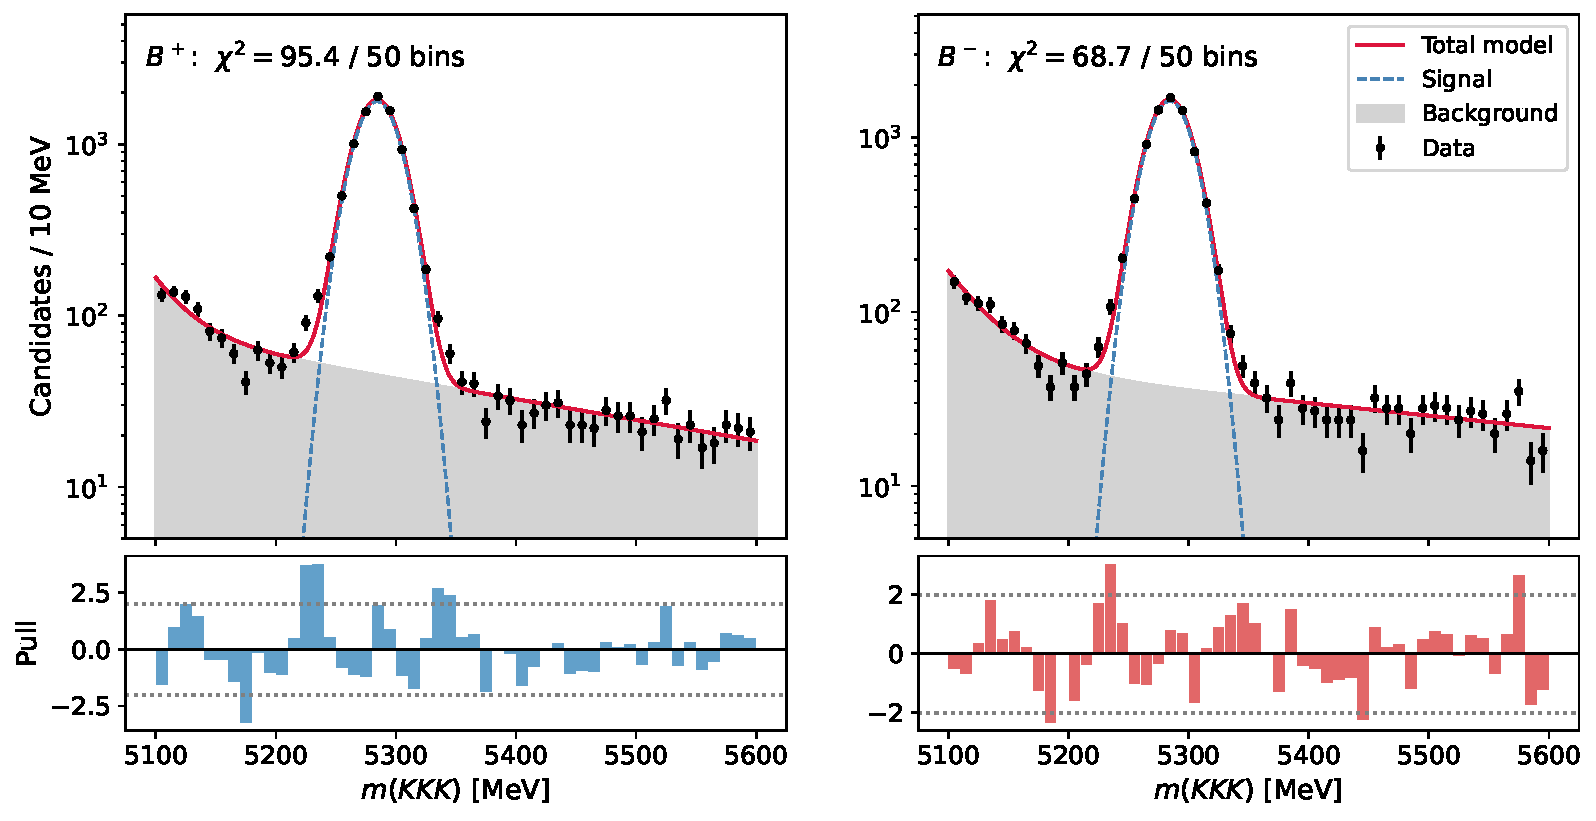
\includegraphics[width=0.8\textwidth]{figures/bayes_nominal_mass_fit.pdf}
\caption{Mass distributions of (a) $B^+$ and (b) $B^-$ candidates with the nominal model (posterior medians, logarithmic scale): total, signal and background components. Bottom: pulls, $(\text{obs}-\text{exp})/\sqrt{\text{exp}}$.}
\label{fig:bayes_fit}
\end{figure*}

\begin{figure*}[t]
\centering
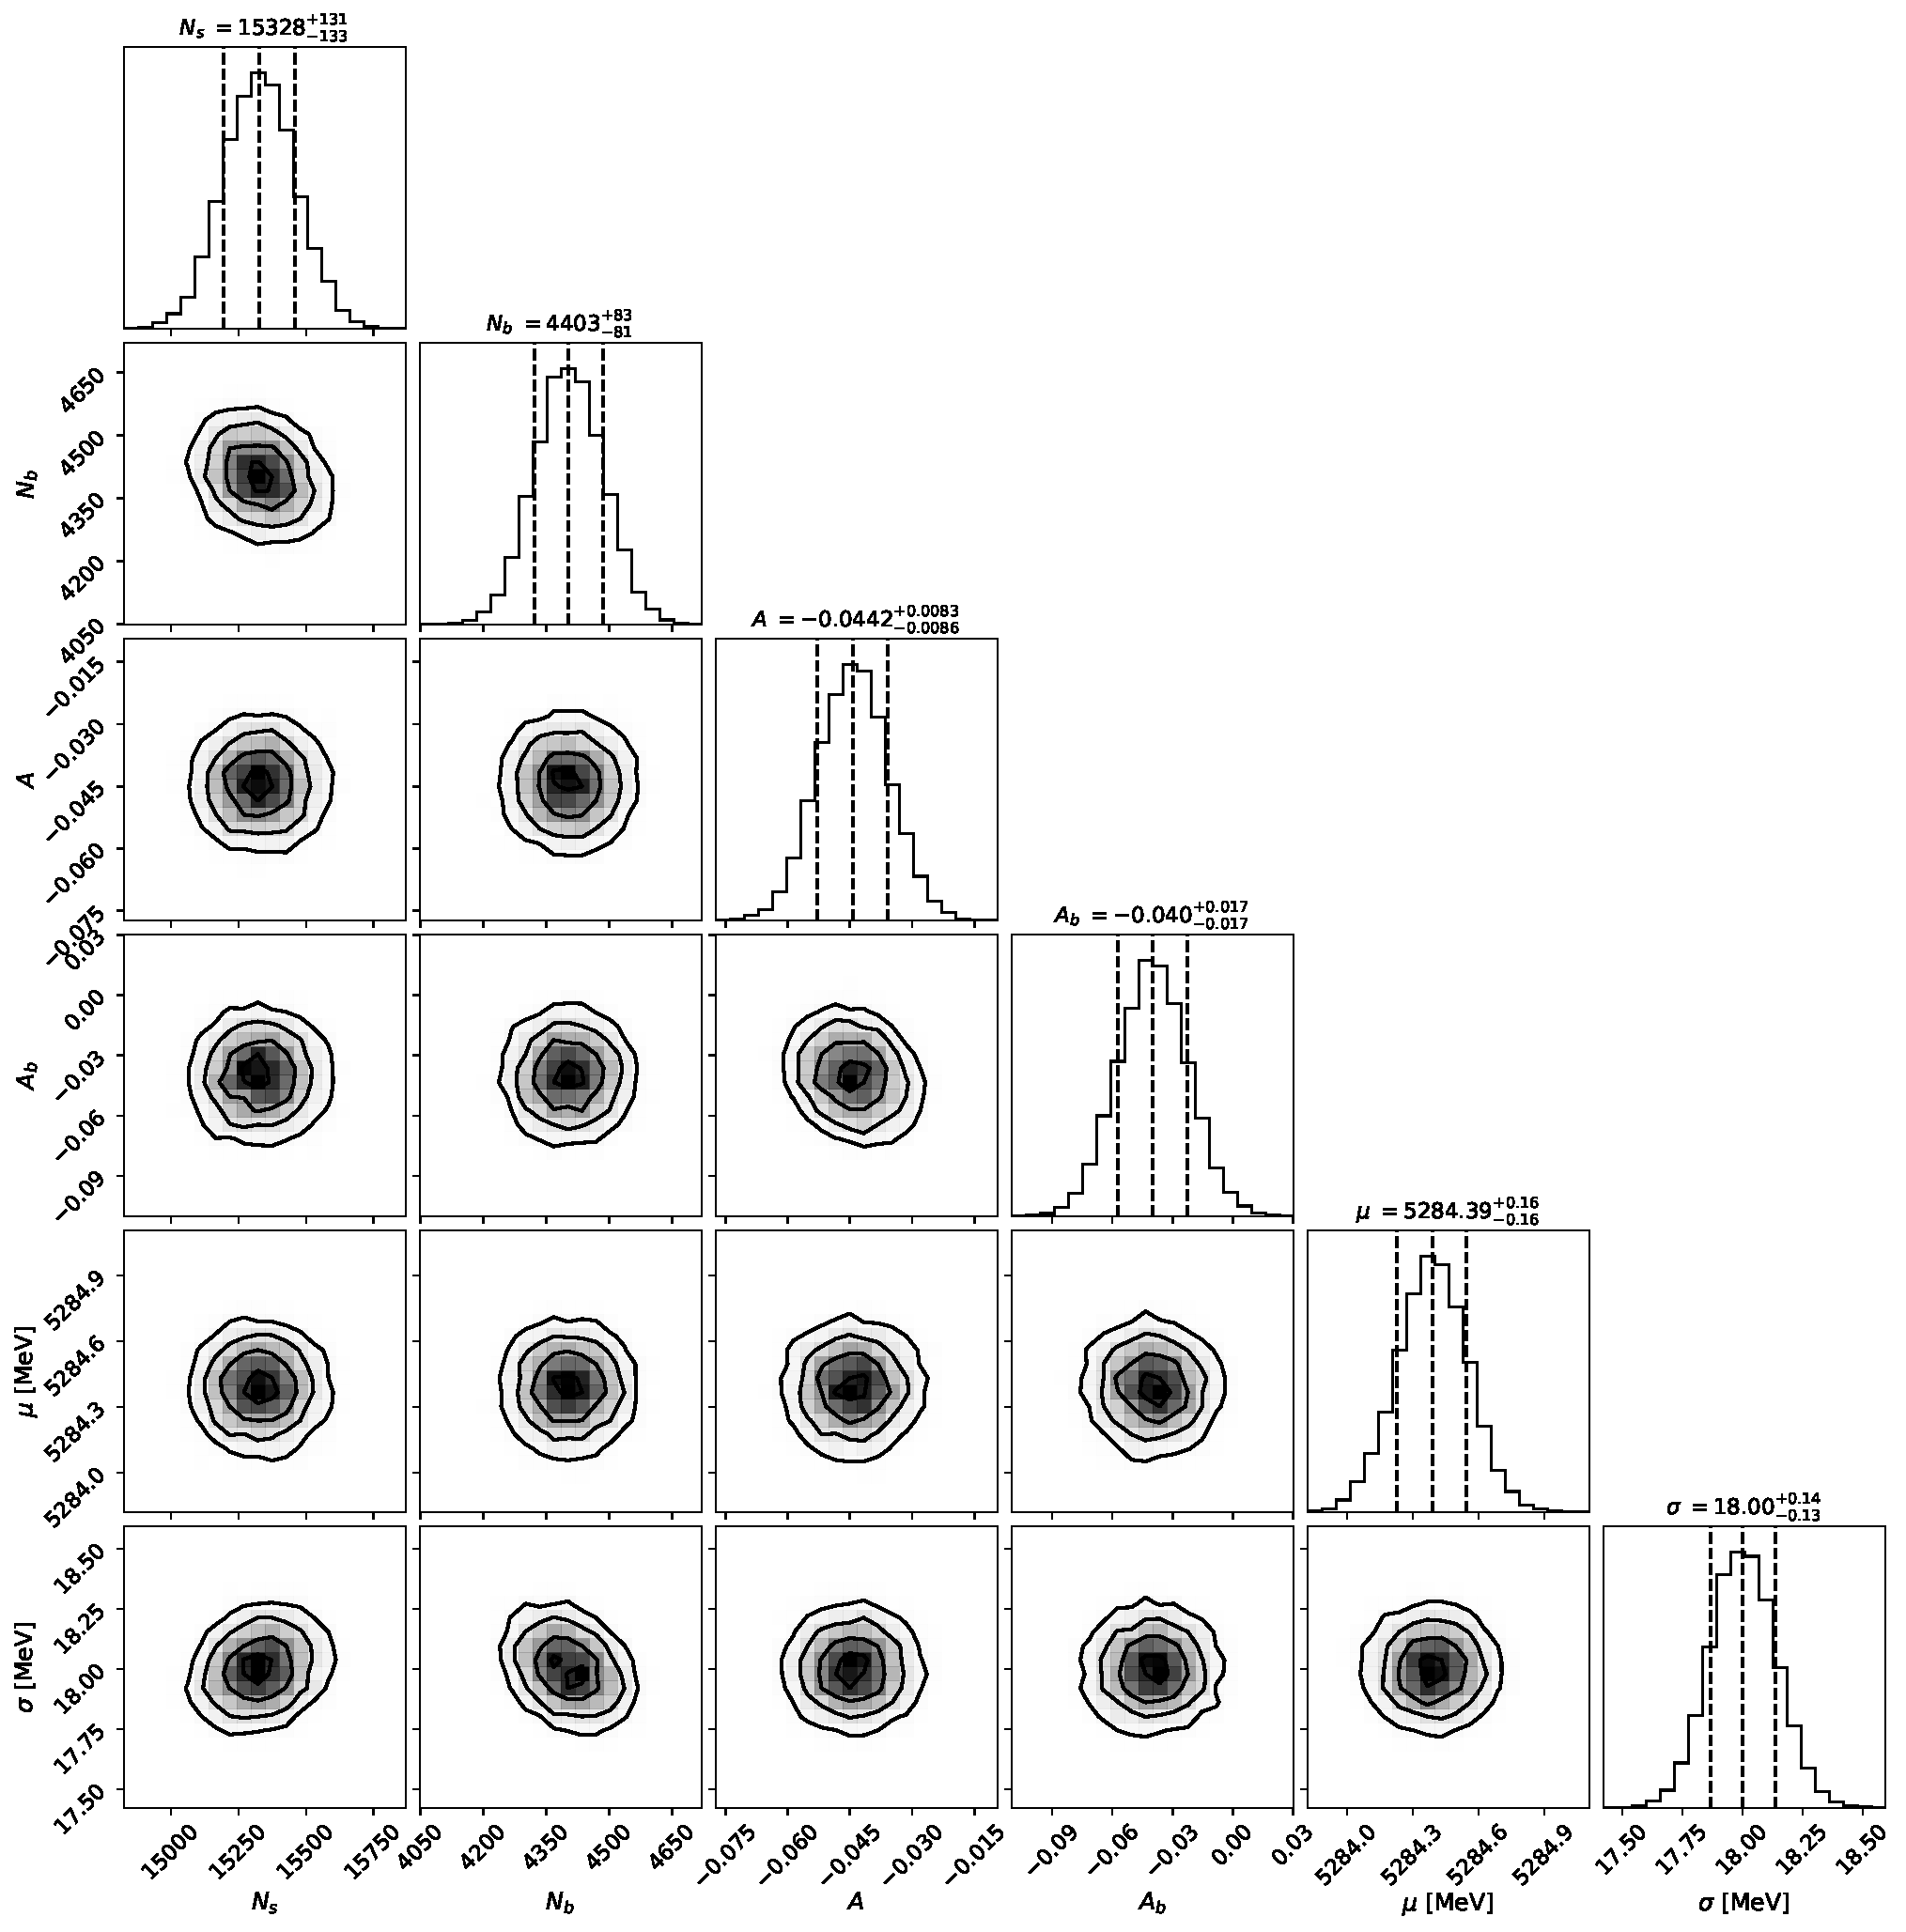
\includegraphics[width=0.55\textwidth]{figures/bayes_nominal_corner.pdf}
\caption{Posterior of the six physics parameters of the nominal fit (the six background-shape parameters are marginalized). Diagonal: marginal posteriors with the 16th, 50th and 84th percentiles (dashed lines and titles). Off-diagonal: 2D marginals, contours enclosing the regions of the $1\sigma$ and $2\sigma$ levels of a 2D Gaussian ($39\%$ and $86\%$).}
\label{fig:bayes_corner}
\end{figure*}

Figure~\ref{fig:bayes_fit} compares the nominal model with the data of the two charges: it follows the spectrum over two orders of magnitude, and the pulls show signal tails heavier than a Gaussian, whose effect on $\Araw$ is negligible (Appendix~\ref{sec:bayes_gof}). The marginal posterior on the raw asymmetry gives (median and equal-tailed credible intervals, CI)
\begin{gather*}
\Araw = -0.0443, \\
68\%~\text{CI}~[-0.0528,-0.0358], \\ 95\%~\text{CI}~[-0.0608,-0.0276].
\end{gather*}
The posterior is very close to Gaussian (standard deviation $0.0085$), so equal-tailed and highest-posterior-density intervals coincide; with uniform priors its mode, $-0.0441$, is the maximum-likelihood estimate and the result can be compared directly with the frequentist fit (Sec.~\ref{sec:frequentist}, Appendix~\ref{sec:appendix_freq}). The other physics parameters (Fig.~\ref{fig:bayes_corner}) are $N_s=15{,}328\pm133$, $N_b=4404\pm82$, $A_b=-0.040\pm0.018$, $\mu=5284.39\pm0.16\,\MeV$ and $\sigma=18.00\pm0.14\,\MeV$. $A$ is almost uncorrelated with them, which is why profiling (frequentist) and marginalizing (Bayesian) the nuisance parameters give the same result; the largest correlation, $-0.17$, is with $A_b$: conditioning on $A_b=0$ moves $A$ to $-0.0475$, as the fit with a charge-symmetric background does ($-0.0471$, Sec.~\ref{sec:syst}).




\subsection{Bayes Factors}
\label{sec:bayes_factor}
\emph{In short: decisive evidence against $A=0$ (Bayes factor $BF_{10}\approx9\times10^3$); the evidence for a background asymmetry is not significant, and depends on the prior width.}

The Bayes factor compares two hypotheses through their evidences, $BF_{10}=P(D\mid H_1)/P(D\mid H_0)$, and requires proper priors. For the nested hypothesis $H_0$: $A=0$ against $H_1$: $A$ free, with shared priors on the other parameters, it reduces to the Savage-Dickey ratio~\cite{dickey1971} (Appendix~\ref{sec:appendix_freq}),
\[
BF_{01} = \frac{p(A=0\mid D)}{\pi(A=0)}, \qquad \pi(A=0)=\tfrac12 .
\]
$A=0$ lies $5.2$ posterior standard deviations from the median, where the chain has essentially no samples, so $p(A=0\mid D)$ was taken from the Gaussian approximation of the marginal posterior: $BF_{01}\approx1.1\times10^{-4}$ ($BF_{10}\approx9\times10^{3}$), decisive evidence against $A=0$ on Jeffreys' scale~\cite{jeffreys}. The value scales with the prior width (Ockham factor): with $A\in(-0.3,0.3)$, $BF_{01}$ drops by a factor $3.3$ and the conclusion is unchanged (Fig.~\ref{fig:checks_bf}; the Savage-Dickey densities are in Fig.~\ref{fig:bayes_sd} of Appendix~\ref{app:ext_bayes}, further checks in Appendix~\ref{sec:checks_profile}).

\begin{figure}[h]
\centering
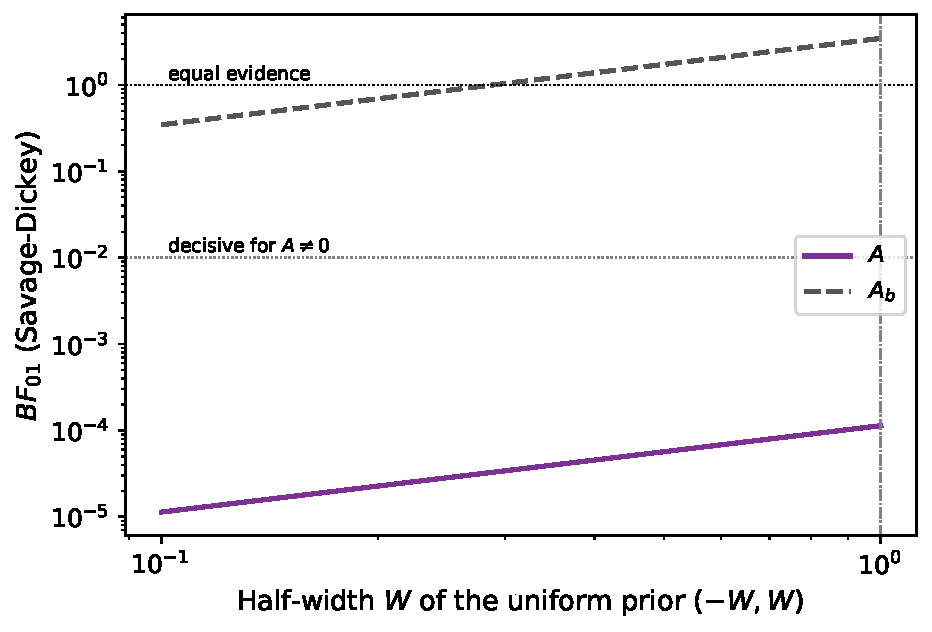
\includegraphics[width=\columnwidth]{figures/validation_bf_prior_width.pdf}
\caption{$BF_{01}$ of $A=0$ and of $A_b=0$ as a function of the half-width $W$ of the uniform prior $(-W,W)$ (Gaussian approximation of the posterior, Savage-Dickey). The vertical line marks the nominal prior.}
\label{fig:checks_bf}
\end{figure}


The same test on the background asymmetry shows the Ockham factor at work: $A_b=-0.040\pm0.018$ is $2.3$ standard deviations from zero, yet $BF_{01}(A_b=0)\approx3.5$, because the likelihood gain does not compensate for spreading the prior over $(-1,1)$; unlike for $A$, the preference changes sign with the prior width (Fig.~\ref{fig:checks_bf}, crossing at $W\approx0.3$). A negative $A_b$ is plausible given the misidentified $B^\pm\to K^\pm\pi^+\pi^-$ and $\pi^\pm K^+K^-$ decays; $A_b$ is kept free in the nominal model and fixing it to zero is one of the systematic variants (Sec.~\ref{sec:syst}).

\paragraph*{Further material} is in Appendix~\ref{app:ext_bayes}. \emph{Model Adequacy: Goodness of Fit and Posterior Predictive Check}: the model does not reach $\chi^2/\mathrm{ndof}\approx1$ ($164.1/88$), mainly because the signal tails are heavier than a Gaussian, but $\Araw$ changes by only $-0.0002$ with a Crystal Ball signal.
